\section{Présentation de R}

\begin{frame}
  \frametitle{Bref historique}

  «\emph{R is a free software environment for statistical computing and graphics}»
  \bigskip

  \begin{itemize}
  \item À l'origine fut le S --- milieu des années 1970 --- John~M.\ Chambers
  \item Principalement popularisé par mise en {\oe}uvre commerciale
    S-PLUS
  \end{itemize}
  \bigskip

  \begin{quote}
    \begin{minipage}{0.35\linewidth}
      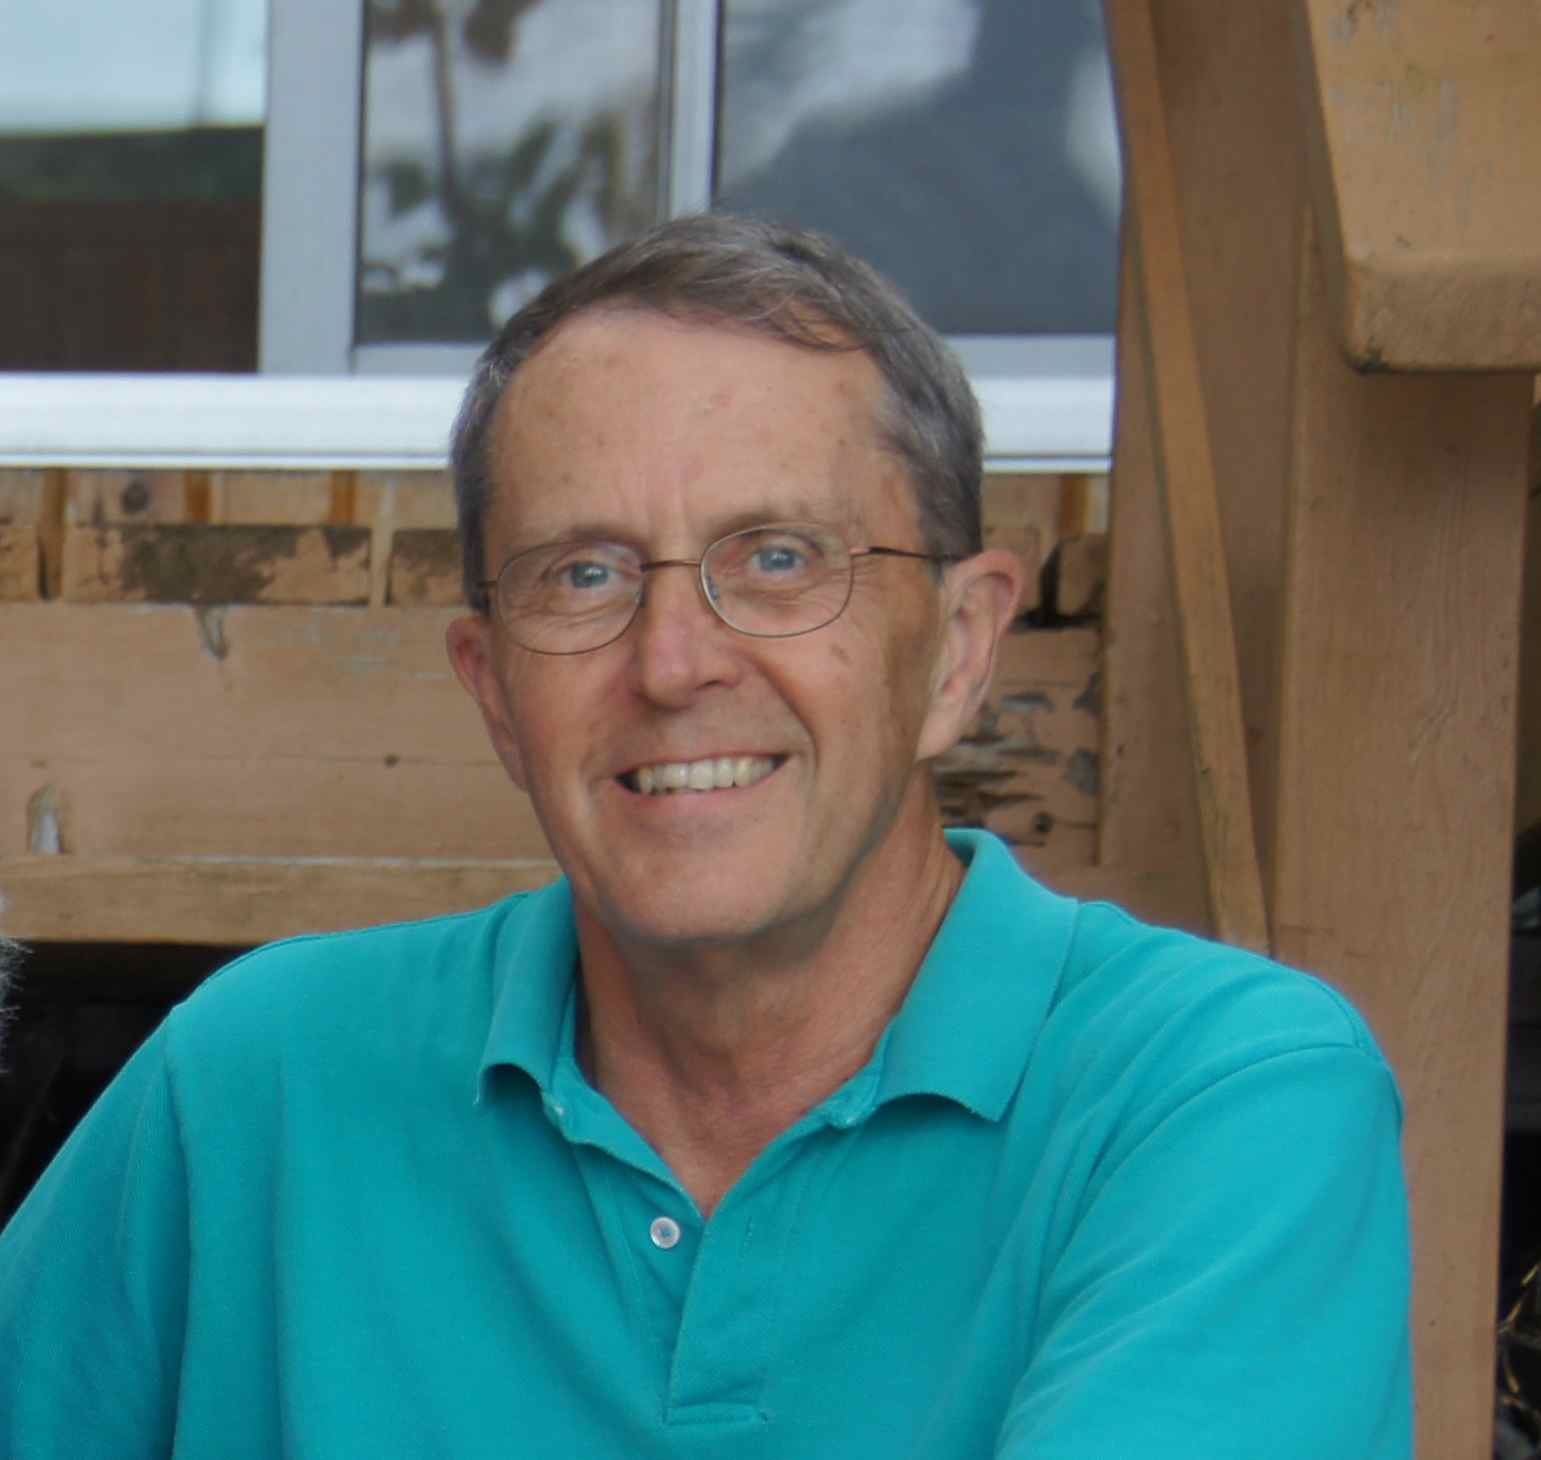
\includegraphics[width=\linewidth,keepaspectratio]{Chambers}
    \end{minipage}
    \hfill
    \begin{minipage}{0.6\linewidth}
      \raggedright
      \textbf{ACM Software System Award 1998} \\
      \emph{John Chambers --- Langage S} \\[\baselineskip]

      «\dots\ which has forever altered how people analyse,
        visualize and manipulate data»
    \end{minipage}
  \end{quote}
\end{frame}

\begin{frame}[fragile=singleslide]
  \frametitle{Bref historique (suite)}

  \begin{itemize}
  \item Nouvelle mise en {\oe}uvre du langage --- milieu des années
    1990 --- \textbf{R}oss Ihaka et \textbf{R}obert Gentleman
  \item Inspirée de Scheme (un dérivé du Lisp) avec syntaxe du S
\begin{Schunk}
\begin{lstlisting}[language=lisp]
(define factorial (lambda (n)
  (if (= n 1)
      1
    (* n (factorial (- n 1))))))
\end{lstlisting}
\end{Schunk}
vs
\begin{Schunk}
\begin{lstlisting}
factorial <- function(n)
  if (n == 1) 1 else n * factorial(n - 1)
\end{lstlisting}
\end{Schunk}
  \item Libre («GNU S») et ouvert (CRAN) --- R surpasse S-PLUS
  \end{itemize}
\end{frame}

\begin{frame}
  \frametitle{Description sommaire de R}

  \begin{itemize}
  \item Environnement intégré de manipulation de données, de calcul et
    de préparation de graphiques
  \item Aussi un langage de programmation complet
    \begin{itemize}
    \item fonctionnalités statistiques de R programmées en R
    \end{itemize}
  \item Langage \emph{interprété} (et non \emph{compilé})
    \begin{itemize}
    \item analogie avec Excel...
    \end{itemize}
  \end{itemize}

  \pause
  \video{https://youtu.be/PSQIKSKw_ys}{Principales caractéristiques du langage R}
\end{frame}

\begin{frame}
  \frametitle{Obtenir de l'aide}

  \begin{alertblock}{Astuce}
    Consulter l'aide en ligne officielle de R.
  \end{alertblock}
\end{frame}

\begin{frame}[fragile=singleslide]
  \frametitle{Obtenir de l'aide (suite)}

  \begin{itemize}
  \item Rubrique d'aide de l'objet \texttt{foo} accessible avec
    \begin{Schunk}
\begin{lstlisting}
?foo
\end{lstlisting}
    \end{Schunk}
    ou
    \begin{Schunk}
\begin{lstlisting}
help(foo)
\end{lstlisting}
    \end{Schunk}
    ou via les interfaces graphiques
  \item Documents plus longs avec
    \begin{Schunk}
\begin{lstlisting}
vignette("`\meta{sujet}'")
\end{lstlisting}
    \end{Schunk}
  \item Documentation officielle de R en six guides
    \begin{itemize}
    \item \emph{An Introduction to R}
    \item \emph{R Data Import/Export}
    \end{itemize}
  \end{itemize}
\end{frame}

\begin{frame}
  \frametitle{Démonstration}
  \begin{itemize}
  \item Interfaces
  \item Stratégies de travail
  \item Éditeurs de texte et environnements intégrés
  \item Anatomie d'une session de travail
  \end{itemize}

  \gotoR{presentation.R}
\end{frame}

%%% Local Variables:
%%% mode: latex
%%% TeX-engine: xetex
%%% TeX-master: "raquebec-atelier-introduction-r"
%%% End:
